\newpage

% =============== OBJETIVOS ===================== %

\section{Objetivos}

Os principais objetivos dessa prática são determinar o calor específico de um sólido e o calor latente de condensação da água, fazendo o uso de um calorímetro com uma capacidade térmica calculada por meio dos experimentos.\\

Desse modo, poderemos entender melhor o funcionamento de um calorímetro e melhorar nossos conhecimentos sobre o tema da calorimetria. \\

% =============== INTRODUÇÃO ===================== %
% \newpage
\section{Introdução}

Vamos considerar dois corpos A e B, com diferentes temperaturas $T_A$ e $T_B$, respectivamente, tais que $T_A > T_B$. Ao colocar os corpos em contato, ocorre uma transferência de calor(energia térmica) do corpo mais quente para o corpo mais frio, ou seja, de A para B. Essa transferência de calor cessa ao atingir o equilíbrio térmico entre os dois
corpos, ou seja, quando suas temperaturas forem iguais $T'_A$ = $T'_B$.\\

A quantidade de calor $Q$ é equivalente à quantidade de energia térmica trocada pelos corpos em questão. Dessa forma, em unidades do sistema internacional (SI), a unidade de quantidade de calor $Q$ é o Joule (J). Por razões históricas, outra unidade é também usada, a caloria (cal), cuja relação com o Joule é: 1 cal = 4,186 J.\\

Agora que explicitamos as unidades utilizadas e o conceito da transferência de calor, podemos partir para os experimentos.\\

\begin{figure}[H]
  \centering
  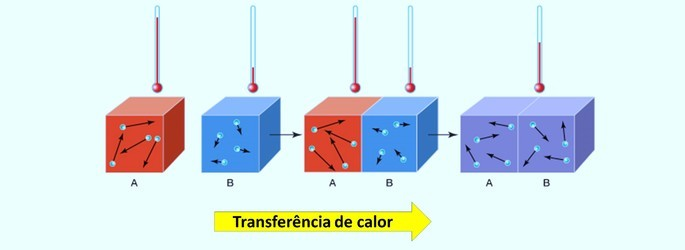
\includegraphics[scale=0.67]{images/Transferencia de calor.jpg}
  \caption{Transferência de calor entre dois corpos com diferentes temperaturas.}
\end{figure}
